\documentclass[12pt]{article}
%\usepackage{times}
\usepackage{graphicx}
\usepackage{array}
\usepackage{float}
%this is a comment
\title{Software Design Specification and User Interface: CommunityConnect}
\author{Kamron Ebrahimi \& Samuel Wilson \& Leif Tsang \\ \& Thomas Korsness  \& Quinton Osborn \\ ebrahimk, wilsosam, tsangl, korsnest, osbornq}
\date{\today}

\begin{document}

\maketitle

\tableofcontents

\newpage
\section{\bf User Interface Prototypes}
  \subsection{\bf UI Prototype One}

        \begin{figure}[H]
                \includegraphics[width =\linewidth,scale=0.5]{UIone.eps}
                \caption{User Interface 1}
                \label{fig: User Interface 1}
        \end{figure}

  \paragraph{\normalfont \indent User interface diagram one \ref{fig: User Interface 1} displays the flowchart for CommunityConnects first user interface prototype. The diagram details the overall web page by we bage flow a user experiences when using CommnuityConnect. The first displayed page is the home page, which consists of a real time map displaying CommunityConnect user concentrations as a heat map. This map is displayed and updated by communicating with a Google maps API. The bottom three fields of the home page allow the user to utilize different functions of CommunityConnect. The far right button allows the user to create a profile with CommunityConnect. The profile creation page has fields for the user to input all required information for CommunityConnect to function properly. If the user already has an established account the “edit profile” page appears containing the information the user previously entered. On this page the user can update or change the information in the profile fields.
  }
  \paragraph{\normalfont \indent The middle button of the home page allows the user to access their previous bookmarked connections. This would be a simple page in which the user could scroll through to see all previous bookmarked connections. The the user can either message an individual through CommunityConnect (an email connected messaging service similar to craigslist), or the user can report an individual if they experienced some form of harassment or behavior which is inconsistent with the CommunityConnect terms of use and guidelines.
  }
  \paragraph{\normalfont \indent The far left field of the home page allows the user to perform a search and find any other users with the same country of origin or interests in the same location. The search page will display a visually pleasing gif while the search algorithm in the server retrieves matches. The server will return all matches, from where the user can select a profile and inspect their information in greater detail.
  }


\newpage
  \subsection{\bf UI Prototype Two}

      \begin{figure}[H]
              \includegraphics[width =\linewidth,scale=0.5]{UItwo.eps}
              \caption{User Interface 2}
              \label{fig: User Interface 2}
      \end{figure}

    \paragraph{\normalfont \indent The second UI prototype is very similar to the first however this implementation has greater function due to specified login and setting pages. The UI implementation also provides a different color scheme, which may be more visually pleasing.
    }
    \paragraph{\normalfont \indent The second UI prototype has a very similar flow of events as the first UI implementation. From the home page, featuring the realtime user concentration map, the user can either perform a search, access their bookmarked connections, or edit their profiles/create a profile. If the user is not logged in none of this functionality is available to the user and he/she will be directed to the login page to enter their credentials. After logging in the user can perform all the same functionality as described in the first UI prototype however the user can also access a dedicated page for configuring the setting of the users account. Some of these settings include changing how the matching algorithm generates matches. For example the user can only have matches based off of their ‘country of origin’ and not interests. The user can also adjust the mile radius from their location matches will be returned from.
    }


  \subsection{\bf UI Prototype Three}

    \begin{figure}[H]
            \includegraphics[width =\linewidth,scale=0.5]{UIthree.eps}
            \caption{User Interface 3}
            \label{fig: User Interface 3}
    \end{figure}

      \paragraph{\normalfont \indent The third UI implementation changes the flow in which the user interacts with CommunityConnect from the first two prototypes. From the home page the user access the functions of CommunityConnect by using the menu button. From the menu the user can access the ‘terms of use’, the website ‘guidelines’ or their profile. This implementation groups CommunityConnect functions by placing the search function and friend list access under the users profile. Like the second UI implementation, if the user is not logged in and attempts to use CommunityConnect functions, he/she will have to login first. If the user doesn't have an account then they will have to create one using the ‘Create Profile’ page. After an account is created the user can search CommunityConnect’s user database for connections, or access their bookmarked connections.
      }

\section{\bf Class Diagram}
      \begin{figure}[H]
              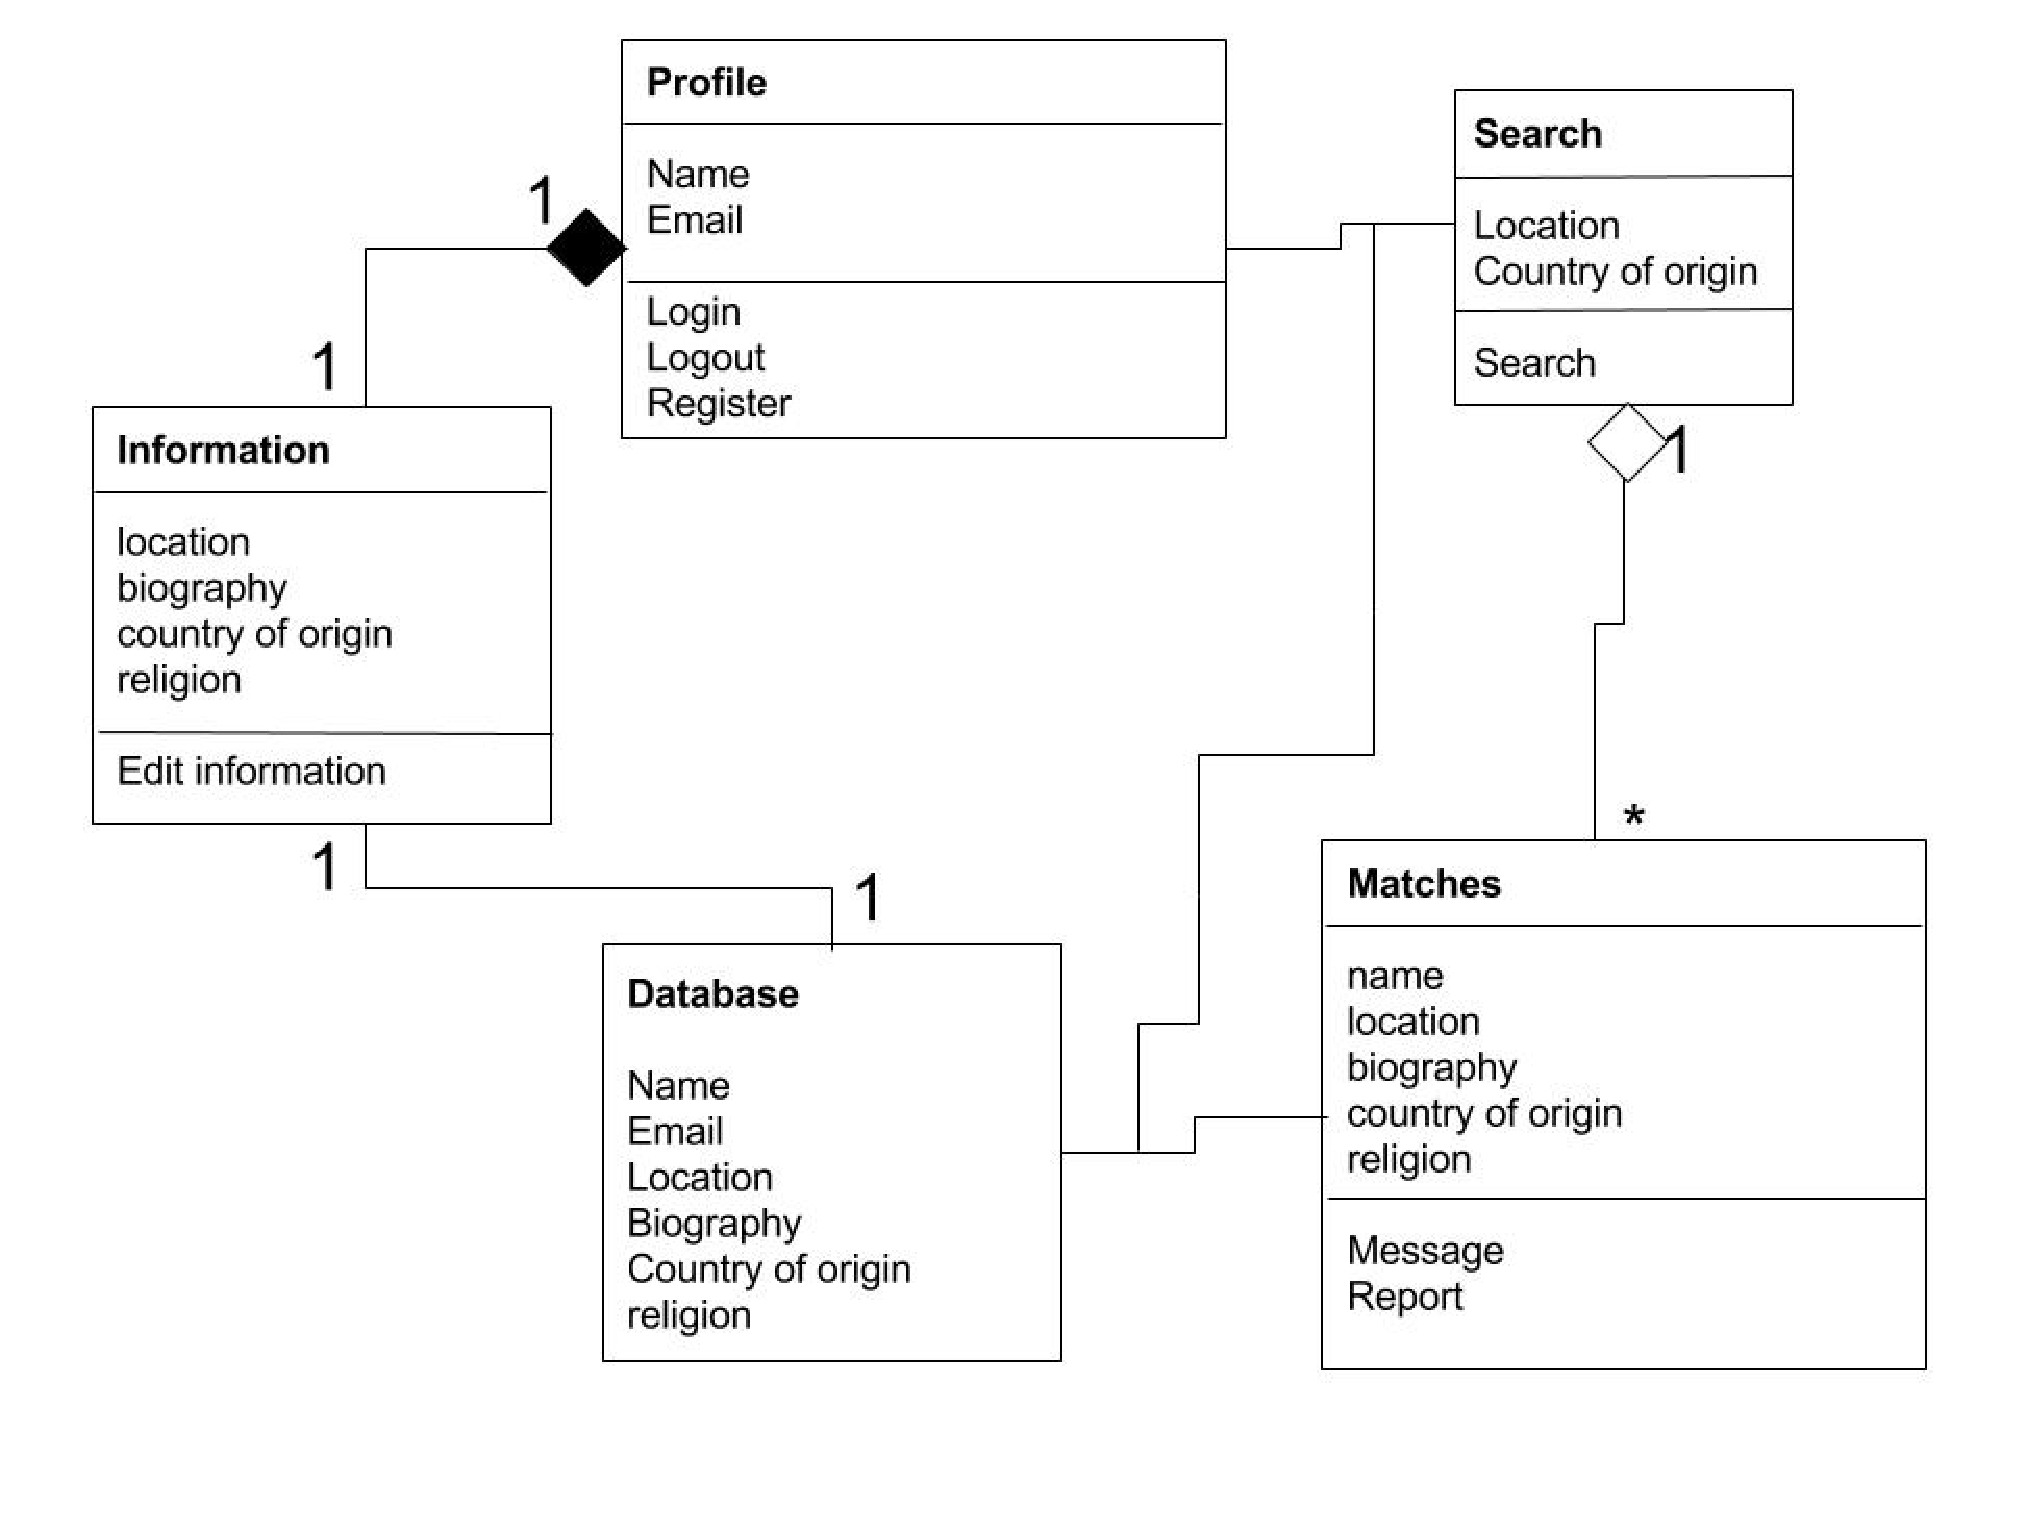
\includegraphics[width =\linewidth]{CC_class_diagram.eps}
                \caption{Class Diagram}
                \label{fig: Class Diagram}
      \end{figure}


\newpage
\section{\bf Sequence Diagrams}
  \subsection{\bf Use Case 1}
      \paragraph{\normalfont \indent During the find friends sequence the user hits the find friends button and the web page will respond by contacting the server with a database of people to see what users should show up on that list. The server returns a list of people to be refreshed onto the list on the web page. The user than views that list and then gets in contact with the second user from utilities on the web page.
      }

      \begin{figure}[H]
              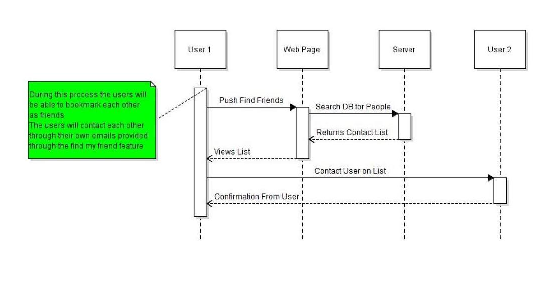
\includegraphics[width =\linewidth]{sequenceDiagram1.eps}
                \caption{Sequence Diagram for Use Case 1}
                \label{fig: Sequence Diagram 1}
      \end{figure}

  \newpage
  \subsection{\bf Use Case 2}
      \paragraph{\normalfont \indent During the editing of the profile the user will press the button to edit the profile and then go to the web page for editing the profile. This page will then validate legit input into another function to contact the server if it passes the validation check. This is sent to and saved on the server and this is repeated each time the settings are changed. Finally the page is saved and the page is exited out of by the user.
      }

      \begin{figure}[H]
              \includegraphics[width =\linewidth]{sequenceDiagram2.eps}
              \caption{Sequence Diagram for Use Case 2}
              \label{fig: Sequence Diagram 2}
      \end{figure}

  \newpage
  \subsection{\bf Use Case 3}

    \paragraph{\normalfont \indent When the user wants to go to the homepage they will hit the homepage button. The web page will then request the permissions to the server in order to see what permissions that user has. The server will send back a set of permissions and the webpage will use that information to construct a basic layout for the web page.
    }

      \begin{figure}[H]
              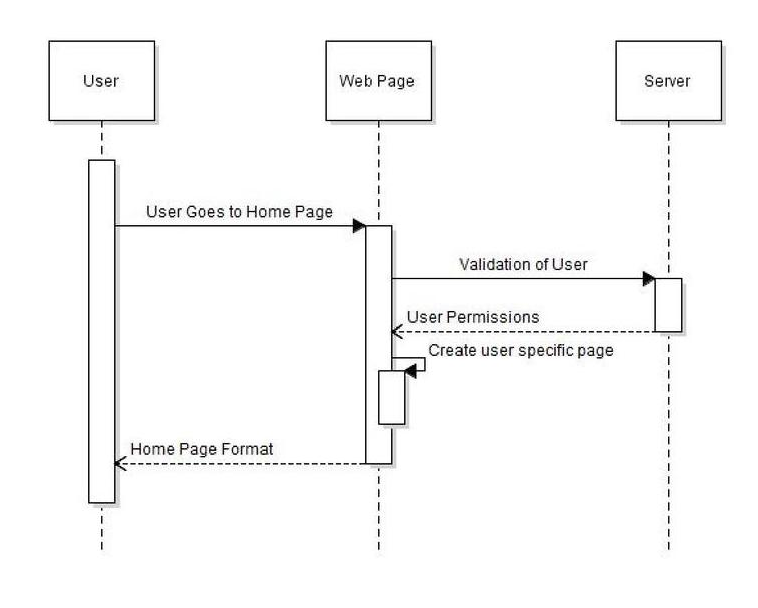
\includegraphics[width =\linewidth]{sequenceDiagram3.eps}
              \caption{Sequence Diagram for Use Case 3}
              \label{fig: Sequence Diagram 3}
      \end{figure}

\section{\bf Meeting Report}
  \paragraph{\normalfont \indent This week we completed the third assignment and got a better understanding of how we will implement our ideas. Our starting and main goal for CommunityConnect is to create a simple platform that allows users to find other people who are nearby and of similar cultural background. Additionally we have begun constructing the homepage of the CommunityConnect website usign HTML and CSS. To complete our project we will need:
  }
   \begin{itemize}
    \item A user profile page.
    \item A search system with a database.
    \item A “matches” page to show profiles returned from the search.
   \end{itemize}

  \paragraph{\normalfont \indent These are the core components which form the core function of our project, but since we are using a spiral production style, we expect that we will have time to implement other features. Some of these include:
  }
   \begin{itemize}
    \item A message system, instead of email.
    \item Group profiles, allowing members to join.
    \item Searches for other tags.
   \end{itemize}

  \paragraph{\normalfont \indent We are unsure what our next assignment will be, but we are ready to begin programming if necessary. We will use the university’s hosting for our website and finding hosting for our database. We may use PHP or NodeJS with Handlebars to make our website dynamically created. Our goal once we begin programming, will be to write each piece of code in a modular fashion, so we are able to easily add new features later.
  }

  \paragraph{\normalfont \indent The customers were able to meet with the team, and have been helping the team. Individually, we worked on:
  }

\begin{center}
\begin{tabular}{ |c|c| }
 \hline
 Kamron Ebrahimi & UI Prototypes and Sketches - LaTex \\
 Quinton Osborn & UI Prototypes and Sketches \\
 Leif Tsang & Sequence Diagrams \\
 Thomas Korsness & Class Diagrams \\
 Samuel Wilson & Class Diagrams - Meeting Report \\
 \hline
\end{tabular}
\end{center}

\end{document}
